\section{Progettazione logica}
\subsection{Stima del volume dei dati}

\subsection{Descrizione delle operazioni principali e stima della frequenza}

\subsection{Schemi di navigazione e tabelle degli accessi}

\subsection{Raffinamento dello schema}
(eliminazione di identificatori esterni, attributi composti e gerarchie, scelta delle chiavi)
(elimanzione dell'attributo composto Position e l'inserimento delle due coordinate)

\subsection{Analisi delle ridondanze}

\subsection{Traduzione di entità e associazioni in relazioni}
players(\textbf{name})\newline

colors(\textbf{hex}, red, green, blue, name)\newline

games(\textbf{id}, server\_id, concluded)\newline
FK: server\_id REFERENCES servers(id)\newline

players\_in\_game(\textbf{player\_name}, \textbf{game\_id}, color\_hex, score, current, order)\newline
FK: player\_name REFERENCES players(name)\newline
FK: game\_id REFERENCES games(id)\newline
FK: color\_hex REFERENCES colors(hex)\newline

games\_expansions(\textbf{expansion\_name}, \textbf{game\_id})\newline
FK: game\_id REFERENCES games(id)\newline
FK: expansion\_name REFERENCES expansions(name)\newline

expansions(\textbf{name})\newline

meeple\_types(\textbf{name}, quantity, strength, expansion\_name)\newline
FK: expansion\_name REFERENCES expansions(name)\newline

meeples(\textbf{id}, owner\_player\_name, owner\_game\_id, type\_name, placed)\newline
FK: owner\_player\_name REFERENCES players\_in\_game(player\_name)\newline
FK: owner\_game\_id REFERENCES players\_in\_game(game\_id)\newline
FK: type\_name REFERENCES meeple\_types(name)\newline

gamesets(\textbf{id}, type\_name, points, closed)\newline
FK: type\_name REFERENCES gameset\_types(name)\newline

gameset\_types(\textbf{name}, starting\_points, endgame\_ratio, expansion\_name)\newline
FK: expansion\_name REFERENCES expansions(name)\newline

tile\_section\_types(\textbf{name}, next\_name*, previous\_name*)\newline
FK: next\_name REFERENCES tile\_section\_types(name)\newline
FK: previous\_name REFERENCES tile\_section\_types(name)\newline

tile\_sections(\textbf{type\_name}, \textbf{tile\_order}, \textbf{tile\_game\_id}, gameset\_id, meeple\_id*, closed)\newline
FK: type\_name REFERENCES tile\_section\_types(name)\newline
FK: tile\_order REFERENCES tiles(order)\newline
FK: tile\_game\_id REFERENCES tiles(game\_id)\newline
FK: meeple\_id REFERENCES meeples(id)\newline
FK: gameset\_id REFERENCES gamesets(id)\newline

tiles(\textbf{order}, \textbf{game\_id}, type\_name, rotation\_count, x\_coordinate*, y\_coordinate*, current)\newline
FK: type\_name REFERENCES tile\_types(name)\newline
FK: game\_id REFERENCES games(id)\newline

tile\_types(\textbf{name}, quantity, expansion\_name)\newline
FK: expansion\_name REFERENCES expansions(name)\newline

tile\_type\_configurations(id, \textbf{tile\_section\_type\_name}, \textbf{tile\_type\_name}, gameset\_type\_name, closed, pennant)\newline
FK: tile\_section\_type\_name REFERENCES tile\_section\_types(name)\newline
FK: tile\_type\_name REFERENCES tile\_types(name)\newline
FK: gameset\_type\_name REFERENCES gameset\_types(name)\newline

regions(\textbf{id}, continent\_name, cardinal\_point\_name*)\newline
FK: continent\_name REFERENCES continents(name)\newline
FK: cardinal\_point\_name REFERENCES cardinal\_points(name)\newline

continents(\textbf{name})\newline

cardinal\_points(\textbf{name})\newline

servers(\textbf{id}, region\_id, active, max\_games)\newline
FK: region\_id REFERENCES regions(id)

\subsection{Schema relazionale finale}
\begin{figure}[hb]
    \centering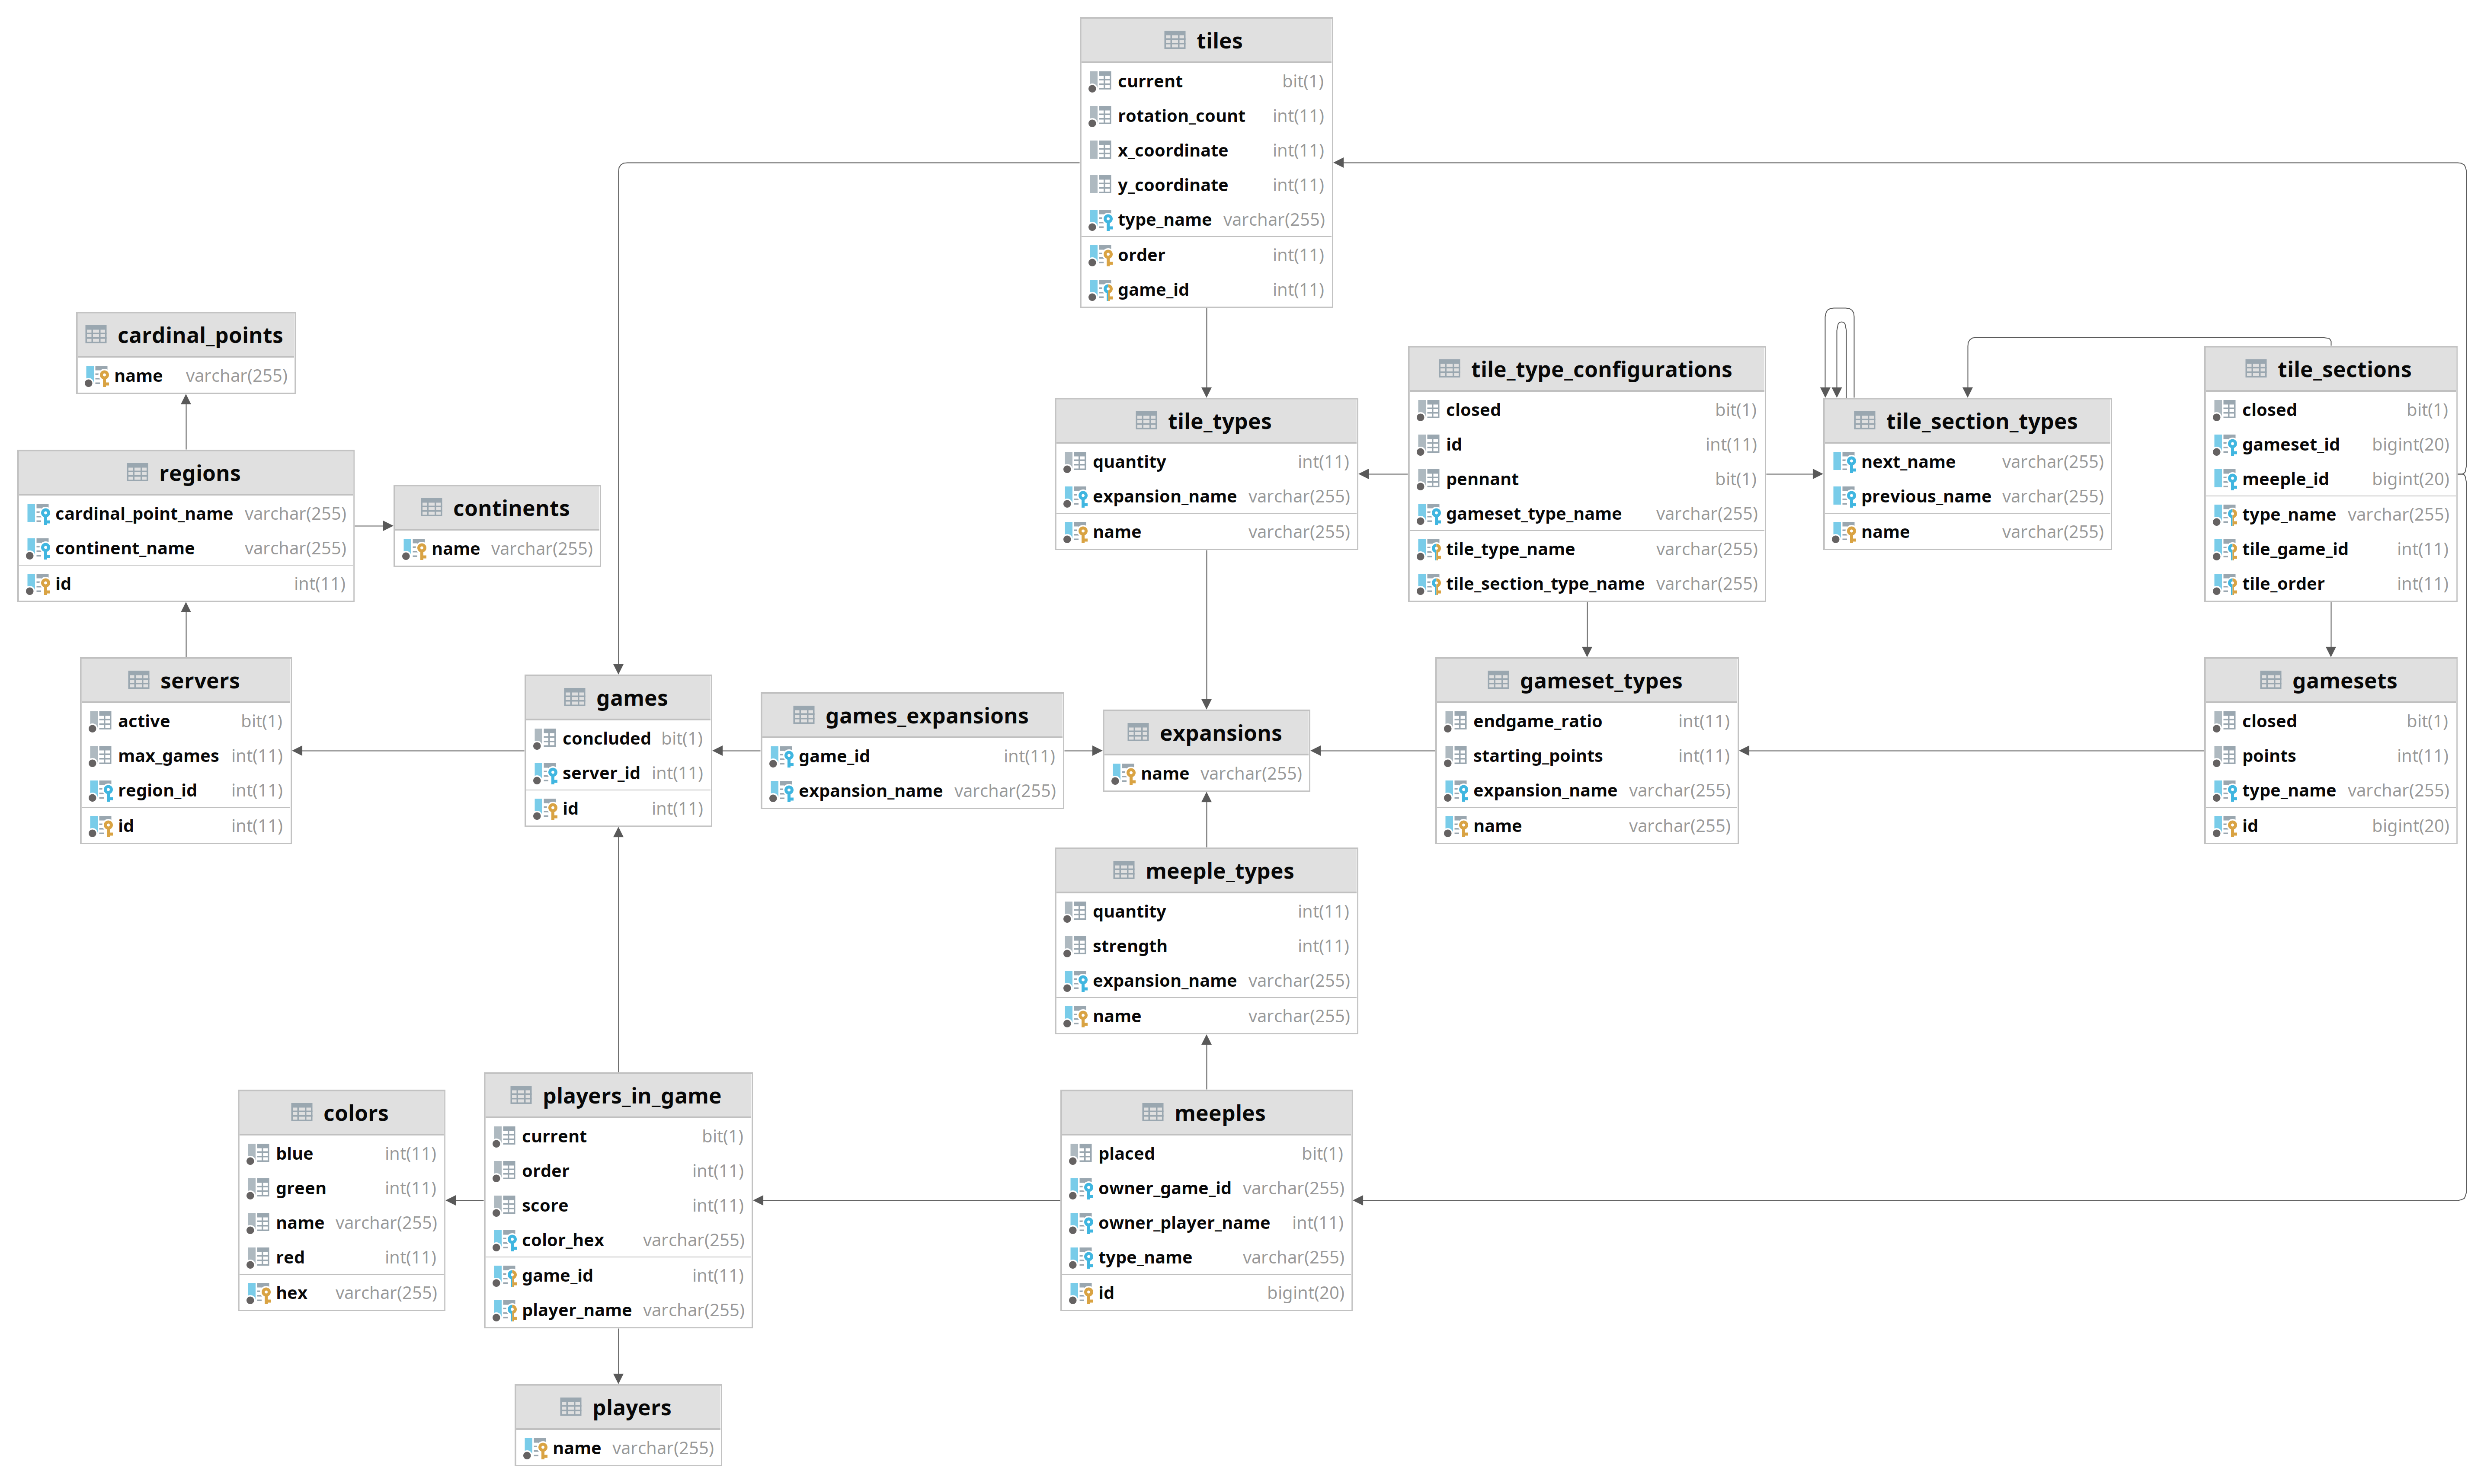
\includegraphics[scale=0.06]{images/Progettazione/relazionale.png}
    \caption{Schema concettuale finale.}
\end{figure}

\subsection{Traduzione delle operazioni in query SQL}
